\documentclass[a4paper, 12pt]{article}

\usepackage[utf8]{inputenc}
\usepackage[T1]{fontenc}
\usepackage[spanish]{babel}
\usepackage[margin=1in, top=1in, bottom=1in, includefoot]{geometry}
\usepackage{graphicx}
\usepackage{fancyhdr}
\usepackage{parskip}
\usepackage{helvet}
\renewcommand{\familydefault}{\sfdefault}
\pagestyle{empty}

\begin{document}

\section*{Encriptación AES (Advanced Encryption
Standard)}\label{encriptaciuxf3n-aes-advanced-encryption-standard}

Como todos los métodos de encriptación, el AES convierte el texto sin
formato en un código que sólo puede descifrar quien tenga la clave.

\textbf{AES} tiene un tamaño fijo de bloque de 128 bits y tamaños de
clave de 128, 192 y 256 bits. Este opera en una matriz de 4x4
\textbf{bytes} llamada \emph{state}.

\subsection*{Tipos de AES}\label{tipos-de-aes}

\begin{itemize}
\item
  \textbf{AES-128}: este método utiliza una longitud de clave de 128 bits para el
  cifrado y el descifrado, lo que da lugar a 10 series de cifrado con
  3,4 x 1038 combinaciones potenciales diferentes.
\item
  \textbf{AES-192}: este método utiliza una longitud de clave de 192 bits para
  cifrar y descifrar, lo que da lugar a 12 series de cifrado con 6,2 x
  1057 combinaciones potenciales diferentes.
\item
  \textbf{AES-256}: este método utiliza una longitud de clave de 256 bits para
  cifrar y descifrar, lo que da como resultado 14 series de cifrado con
  1,1 x 1077 combinaciones potenciales diferentes.
\end{itemize}

\subsection*{Pasos del sistema AES}\label{pasos-del-sistema-aes}

\begin{enumerate}
\def\labelenumi{\arabic{enumi}.}

\item \textbf{Inicialización de claves}: Primero, se selecciona una clave de cifrado de longitud adecuada (128, 192 o 256 bits). Esta clave se usa tanto para cifrar como para descifrar los datos.

\item \textbf{SubBytes}: Cada byte del bloque de datos se sustituye por otro byte según una tabla de búsqueda (S-Box). Esto confunde los datos y dificulta su análisis.

\begin{center}
  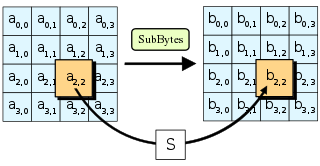
\includegraphics[width=0.4\textwidth]{images/SubBytes.png}
\end{center}

\item \textbf{ShiftRows}: Los bytes en las filas del bloque de datos se desplazan circularmente hacia la izquierda. Esto mezcla los datos y evita patrones predecibles.

\begin{center}
  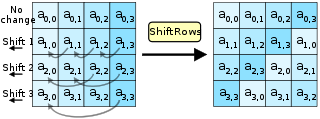
\includegraphics[width=0.4\textwidth]{images/ShiftRows.png}
\end{center}

\item \textbf{MixColumns}: Cada columna del bloque de datos se transforma mediante una operación algebraica. Esto proporciona una difusión adicional de los datos.

\begin{center}
  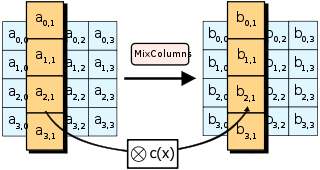
\includegraphics[width=0.4\textwidth]{images/MixColumn.png}
\end{center}

\item \textbf{AddRoundKey}: Se realiza una operación XOR entre el bloque de datos y una subclave derivada de la clave principal para esa ronda. Esto añade una nueva capa de seguridad.

\begin{center}
  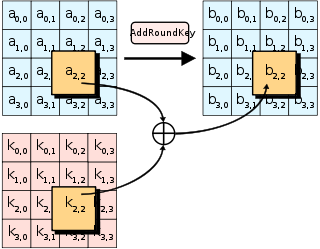
\includegraphics[width=0.4\textwidth]{images/AddRoundKey.png}
\end{center}

\end{enumerate}

El algoritmo AES opera en rondas. Cuantas más rondas, más seguro es el cifrado. El número de rondas depende del tamaño de la clave: 10 rondas para AES-128, 12 rondas para AES-192 y 14 rondas para AES-256. Por lo que estos pasos se realizarán cierta cantidad de veces dependiendo del tamaño de la clave.

\end{document}
